---
title: "泛函分析作业250915"
date: 2025-09-15
collections: "泛函分析作业"
tags: ["泛函分析"]
categories: ["泛函分析"]
---
\problem[1.1.2] (Newton 法) 设 $f$ 是定义在 $[a,b]$ 上的二次连续可微的实值函数, $\hat{x}\in(a,b)$ 使得 $f(\hat x)=0, f'(\hat x)\neq 0$. 求证: 存在 $\hat x$ 的邻域 $U(\hat x)$, 使得 $\forall x_0\in U(\hat x)$, 迭代序列 $$x_{n+1}=x_n-\frac{f(x_n)}{f'(x_n)}\quad (n=0,1,2,\ldots)$$ 是收敛的, 并且 $$\lim\limits_{n\to\infty}x_n=\hat x.$$


\begin{proof}
	设映射 $T(x)=x-\dfrac{f(x)}{f'(x)}$

	由 $f\in C^2, f'(\hat x)\neq 0$, 故存在 $\delta_0, (x-\delta_0,x+\delta_0)\subset[a,b],m,M,L\in\R,\ s.t.\ |x-\hat x|\leqslant \delta_0$ 时, 有 $m\overset{\text{保号性}}{\leqslant}|f'(x)|\overset{\text{有界性}}{\leqslant} M, |f''(x)|\leqslant L$.

	那么考虑导数 $T'(x)=\dfrac{f(x)f''(x)}{(f'(x))^2}\overset{\text{柯西中值}}{=}\dfrac{(f'(\xi)|x-\hat x|+f(\hat x))f''(x)}{(f'(x))^2}\leqslant \dfrac{M|x-\hat{x}|L}{m^2}$, 于是可以取 $\delta=\min(\frac {m^2}{ML+1},\delta_0)$, 则有 $|T'(x)|\leqslant \frac{ML}{ML+1}<1,\ \forall x\in (\hat x-\delta,\hat x+\delta)$.

	所以在该邻域中有 $|T(x)-T(y)|\leqslant \frac{ML}{ML+1}|x-y|,\ \forall x,y\in (\hat x-\delta,\hat x+\delta)$, 再结合 $T(\hat{x})=\hat x$ 可以得到 $Tx\in(\hat x-\delta,\hat x+\delta)$, 即 $T$ 在该邻域内是压缩映射.

 	又由实数的完备性, 根据 Banach 不动点定理可知存在唯一的不动点, 又 $\hat x=T(\hat x)$, 所以 $\hat x$ 是不动点, 即 $\lim\limits_{n\to\infty}x_n=\hat x$.

下面是 Mworks 程序.
\begin{lstlisting}[language=c++]
clear()
clc()

f(x)=exp.(x).-2 #求此函数的零点
df(x)=exp.(x)   #此函数的导数

#绘制f的函数图像
t=0:0.1:1.1
plot(t,f(t),"k")
hold("on")

#绘制直线y=0
plot(t,zeros(size(t)),"r")

x0=0   #初始猜测
N=3    #总迭代次数
x=zeros(1,N+1)
x[1]=x0;
for ii=1:N
x[ii+1]=x[ii]-f(x[ii])/df(x[ii])
text(x[ii],f(x[ii]),string(ii-1),color="black",fontsize=14)
plot(x[ii:ii+1],f(x[ii:ii+1]),"b")
plot(x[ii+1],f(x[ii+1]),"r*")
end
text(x[N+1],f(x[N+1]),string(N),color="black",fontsize=14)
saveas(gcf(),"1d1d2.eps")
[x;
abs.(x.-log(2))] #零点为log(2)
\end{lstlisting}

\begin{figure}[H]
	\centering
	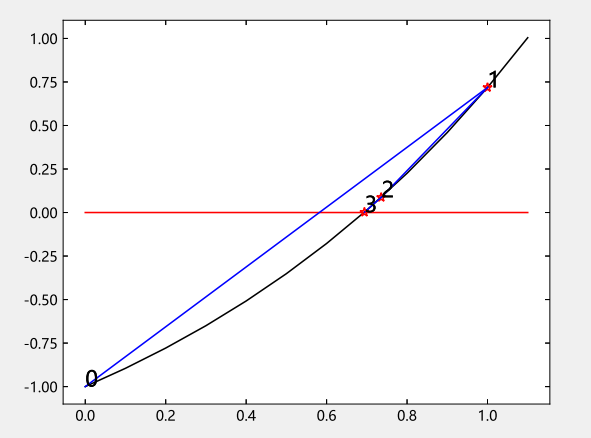
\includegraphics[width=0.8\textwidth]{figures/泛函/1.1.2.png}
\end{figure}
\end{proof}

\problem[1.1.4] 设 $T$ 是度量空间上的压缩映射, 求证: $T$ 是连续的.

\begin{proof}
	记度量空间为 $(\mathscr X,\rho)$.

	设 $\{x_n\}_{n=1}^\infty$ 是该度量空间上的任意收敛列, 且收敛至 $x_0$. 那么对于 $\rho(Tx_n,Tx_0)$, 由于 $T$ 是压缩映射, 故存在 $0<\alpha<1$ 满足 $\rho(Tx,Ty)\leqslant\alpha\rho(x,y),\ \forall x,y\in\mathscr X$, 于是 $0\leqslant\rho(Tx_n,Tx_0)\leqslant\alpha\rho(x_n,x_0)$, 根据夹逼准则可知 $\rho(Tx_n,Tx_0)\to 0\ (n\to \infty)$, 所以 $T$ 是连续的.
\end{proof}

\problem[1.1.5] 设 $T$ 是压缩映射, 求证: $T^n(n\in\N_+)$ 也是压缩映射, 并说明逆命题不一定成立.

\begin{proof}
	记度量空间为 $(\mathscr X,\rho)$.

	由 $T$ 是压缩映射, 所以存在 $0<\alpha<1$, 满足 $\rho(Tx,Ty)\leqslant\rho(x,y),\ \forall x,y\in \mathscr X$. 于是有 $\rho(T^nx,T^ny)\leqslant\alpha\rho(T^{n-1}x,T^{n-1}y)\leqslant\cdots\leqslant\alpha^n\rho(x,y)$, 由 $0<\alpha<1$, 所以 $0<\alpha^n<1$. 又 $T$ 将 $\mathscr X$ 映到自身, 所以经过 $n$ 次后仍映到自身. 从而 $T^n$ 也是压缩映射.

	逆命题不一定成立, 存在反例如下:

	在 [0,1) 中用 $|x-y|$ 做度量, 考虑 $T(x)=\frac{1+\sqrt{3}}{6}x^3$.

	显然 $T$ 将 $[0,1)$ 映到 $[0,1)$

	由 $T'(x)=\frac{1+\sqrt{3}}{2}x^2$, 存在 $x$ 使得 $T'(x)>1$, 故 $T$ 不是压缩映射.

	但由链式法则 $(T^2(x))'=\frac{(1+\sqrt 3)^4}{144}x^8<1,\forall x\in [0,1)$, 从而 $T^2$ 是压缩映射.

	注: 上述构造思考过程如下,

	考虑在 $[0,1)$ 上构造 $T'(x)>1,(T^2(x))'=T'(T(x))\cdot T(x)<1$, 取 $T$ 为简单的幂函数 $cx^k$. 可以推出限制 (在 $x=1$ 成立再结合连续性即可) $\left\lbrace\begin{array}{c}
		ck>1 \\
		ckc^{k-1} ck<1
	\end{array}\right.$ 即 $\left\lbrace\begin{array}{c}
	c>\frac 1 k \\
	c<\sqrt[k+1]{\frac{1}{k^2}}
	\end{array}\right.$ 上述案例取 $k=3$ (因为开 4 次根号比较好看), 并选取 c 为中间值.
\end{proof}


\problem[1.1.6] 设 $M$ 是 $(\R^n,\rho)$ 中的有界闭集, 映射 $T:M\to M$ 满足: $\rho(Tx,Ty)<\rho(x,y)(\forall x,y\in M,x\neq y)$, 求证: $T$ 在 $M$ 中存在唯一的不动点.

\begin{proof}
	由 $\rho(Tx,Ty)<\rho(x,y)$ 和三角不等式可得 $$|\rho(x,Tx)-\rho(y,Ty)|\leqslant \rho(x,y)+\rho(Tx,Ty)<2\rho(x,y),$$ 从而 $\rho(x,Tx)$ 是连续的.

	由于 $M$ 是 $\R^n$中的有界闭集, 所以存在最小值点 $x_0$, 使得 $\rho(x_0,Tx_0)$ 是最小的. 如果 $\rho(x_0,Tx_0)=0$ 那么 $x_0$ 就是不动点.

	反之, 如果 $\rho(x_0,Tx_0)>0$, 那么 $\rho(Tx_0,T^2x_0)<\rho(x_0,Tx_0)$, 从而 $Tx_0$ 更小, 与 $x_0$ 是最小值点矛盾.

	而不动点的唯一性和压缩映像原理相同, 假设有两个不动点, 那么 $\rho(x_0,x_1)=\rho(Tx_0,Tx_1)<\rho(x_0,x_1)$, 矛盾.

	综上, $T$ 在 $M$ 中存在唯一不动点.

	注: 在度量空间中的连续要转变思维用度量去衡量, 即在取 $\delta$ 时, 是对 $\rho(x,x')$ 的限制. 注意区分度量在欧式距离中的连续, 和度量空间中的连续.
\end{proof}

\problem[1.1.7]  对于积分方程 $$x(t)-\lambda\int_0^1 e^{t-s}x(s)\td s=y(t),$$ 其中 $y(t)\in C[0,1]$ 为给定函数, $\lambda$ 为常数, $|\lambda|<1$, 求证: 存在唯一解 $x(t)\in C[0,1]$.


\begin{proof}

考虑度量 $\rho(f,g)=\max\limits_{t\in[0,1]}|f(t)-g(t)|$.

对积分方程做变换得到 $e^{-t}x(t)-\lambda\mint[0]^1 e^{-s}x(s)\td s=e^{-t}y(t)$.

不妨设 $\varphi(t)=e^{-t}x(t),\ \psi(t)=e^{-t}y(t)$, 新的函数显然仍属于 $C[0,1]$, 那么方程变为 $\varphi(t)=\lambda\mint[0]^1 \varphi(s)\td s+\psi(t)$.

考虑映射 $T(\varphi)=\psi+\lambda\mint[0]^1 \varphi\td s$.

首先, 由 $\psi\in C[0,1]$, 所以 $T(\varphi)\in C[0,1]$, 映射到自身.

其次, 对于任意两个属于 $C[0,1]$ 的函数 $f,g$.

$$\rho(Tf,Tg)\overset{\text{差为常数}}{=}\lambda\int_0^1 |f(t)-g(t)|\td t\leqslant\lambda\max\limits_{t\in[0,1]}|f(t)-g(t)|=\lambda\rho(f,g)$$

所以 $T$ 是压缩映射, 故根据压缩映像原理新方程具有唯一解, 又乘 $e^{-t}$ 是双射, 故原方程也在 $C[0,1]$ 上有唯一解.

下面是 Mworks 程序.
\begin{lstlisting}
clear()
clc()

n=20; #离散节点总数
t=1/(2*n):1/n:1-1/(2*n) #居中节点

iter=5 #总迭代次数
x=zeros(n,iter+1)
plot(t,x[:,1],"b*",linewidth=4) #绘制初始猜测(蓝色点)
hold("on")
text(t[end],x[end,1],string(0),color="black",fontsize=14)
lambda=0.5
y=(1-lambda).*exp.(t)
for ii=1:iter
x[:,ii+1]=lambda/n*exp.(t .- transpose(t))*x[:,ii]+y
color_value=2*ii/iter-1 #取值范围调整为-1 到 1, 为使线段颜色可以rgb插值渐变
if color_value>0
plot(t,x[:,ii+1],color=[color_value,1-color_value,0]) #绘制此步结果
else
plot(t,x[:,ii+1],color=[0,1+color_value,-color_value]) #绘制此步结果
end
text(t[end],x[end,ii+1],string(ii),color="black",fontsize=14)
end
x_true=exp.(t)
plot(t,x_true,"r*",linewidth=4) #绘制精确结果(红色点)
saveas(gcf(),"1d1d7.eps")
[x x_true]
\end{lstlisting}

\begin{figure}[H]
	\centering
	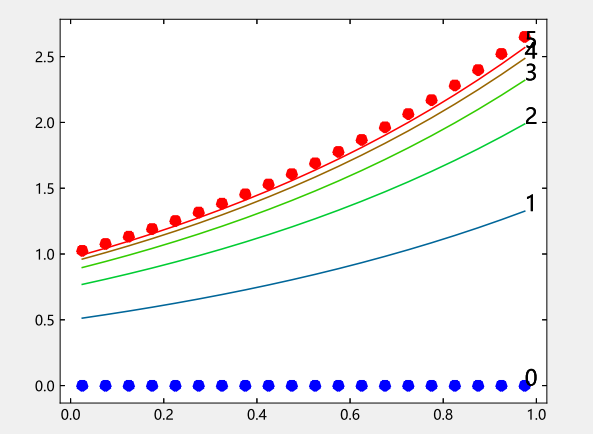
\includegraphics[width=0.8\textwidth]{figures/泛函/1.1.7.png}
\end{figure}
\end{proof}